% !TeX spellcheck = de_DE
\documentclass[
	oneside,  % falls doppelseitiger Druck gewünscht, "oneside" durch "twoside" ersetzen
	ngerman, 
	final, 
	11pt, 
	a4paper, 
	1.1headlines, 
	headinclude=false, 
	footinclude=false, 
	mpinclude=false, 
	pagesize, 
	onecolumn, 
	titlepage, 
	parskip=half, 
	headsepline, 
	chapterprefix=false, 
	version=first, 
	listof=totoc, 
	bibliography=totoc, 
	toc=graduated, 
	fleqn
]{scrbook}

%%%%%%%%%%% Verwendete Pakete %%%%%%%%%%%
\usepackage[T1]{fontenc}
\usepackage[utf8]{inputenc}
\usepackage{babel}
\usepackage{hyperref}
\usepackage[table]{xcolor}
\usepackage{booktabs}
\hypersetup{
	colorlinks=true,
	linkcolor=black,
	urlcolor=black,
	linktoc=all,
	citecolor=black
}
\usepackage{float}
\usepackage{graphicx}
\usepackage{textpos} 
\usepackage{tocloft}
\usepackage{lipsum}
\usepackage{color}
\usepackage[onehalfspacing]{setspace}
\usepackage{acronym}
\usepackage{multicol}
\usepackage{url}

% Einbindung und Konfiguration von nomencl für Nomenklaturen
\usepackage{nomencl}

\renewcommand{\nomname}{Abkürzungsverzeichnis}

\providecommand{\printnomenclature}{\printglossary}
\providecommand{\makenomenclature}{\makeglossary}
\makenomenclature

% Einbindung und Konfiguration von listings für Quellcode-Listings
\usepackage{listings}

\renewcommand\lstlistlistingname{Quellcodeverzeichnis}
\renewcommand{\lstlistingname}{Quellcode}

\definecolor{default-lst-background}{RGB}{242,242,242}
\definecolor{default-lst-keyword}{RGB}{94,20,64}
\definecolor{default-lst-string}{RGB}{15,26,250}
\definecolor{default-lst-comment}{RGB}{31,97,46}

\definecolor{eclipse-java-background}{RGB}{235,235,235}
\definecolor{eclipse-java-keyword}{RGB}{127,0,85}
\definecolor{eclipse-java-string}{RGB}{42,0,255}
\definecolor{eclipse-java-comment}{RGB}{63,127,95}
\definecolor{eclipse-java-annotation}{RGB}{127,159,191}

\lstset{
	basicstyle={\footnotesize\fontfamily{pcr}\selectfont},
	backgroundcolor=\color{default-lst-background},
	keywordstyle=\color{default-lst-keyword}\bfseries,	
	stringstyle=\color{default-lst-string},
	commentstyle=\color{default-lst-comment}\itshape,
	frame=single,
	numbers=left,
	captionpos=b,
	showstringspaces=false,
	breaklines=true,
	tabsize=2
}

%% Listing-Style für Java, der das Syntax Highlighting wie in Eclipse vornimmt
\lstdefinestyle{eclipse-java}{	
	backgroundcolor=\color{eclipse-java-background},
	keywordstyle={\color{eclipse-java-keyword}\bfseries},
	stringstyle={\color{eclipse-java-string}},
	commentstyle={\color{eclipse-java-comment}},		
	moredelim={[il][\textcolor{eclipse-java-annotation}]{\%}},
	moredelim={[is][\textcolor{eclipse-java-annotation}]{\%\%}{\%\%}}
}

%%%%%%%%%%% Weitere Konfigurationen %%%%%%%%%%%
% Schachtelungstiefe
\setcounter{secnumdepth}{3}
\setcounter{tocdepth}{3}

% Schriftart
\makeatletter
\setkomafont{disposition}{\normalcolor\bfseries}
\makeatother

% Balkenfarbe Titelseite
\definecolor{titlepage-rule-color}{RGB}{194,191,194}

%%%%%%%%%%% Angaben zur Arbeit und Autorinnenschaft %%%%%%%%%%%
% Angaben zu Ihrer Arbeit. Bitte ersetzen Sie die Werte der Makros durch die passenden.
%% Art der Arbeit. Gültige Werte: "Projektarbeit", "Bachelorthesis", "Masterseminar", "F\&E-Arbeit", "Masterthesis".
\newcommand*{\fhdopaperkind}{Bachelor Thesis}
%% Titel
\newcommand*{\fhdopapertitle}{Konzeption und Implementierung einer Model-to-Model Transformation zur Überführung unterspezifierter Domänenmodelle in Micoservices}
%% optionaler Untertitel, der etwas länger als der Titel sein kann
\newcommand*{\fhdopapersubtitle}{}
%% Datum der Abgabe im Format DD.MM.YYYY
\newcommand*{\fhdopaperdate}{26.08.2018}
%% erste Betreuerin
\newcommand*{\fhdopaperfirstsupervisor}{Prof. Dr. Sabine Sachweh} 
%% zweite Betreuerin inklusive Abschluss, also z. B. "B.Sc." oder "M.Sc."
\newcommand*{\fhdopapersecondsupervisor}{Florian Rademacher, M. Sc.}

% Angaben zu Ihnen als Autorin. Bitte ersetzen Sie die Werte der Makros durch die passenden.
%% vollständiger Name
\newcommand*{\fhdopaperauthor}{Till Paplowski}
%% Geburtstag
\newcommand*{\fhdopaperbirthday}{09.03.1995}
%% Matrikelnummer
\newcommand*{\fhdopaperstudentnumber}{7090903}
%% Studiengang
\newcommand*{\fhdopapermajor}{Software und Systemtechnik}
%% Der durch Ihren Studiengang angestrebte Abschluss. Gültige Werte: "Bachelor", "Master".
\newcommand*{\fhdopaperdegree}{Bachelor of Science} 

\begin{document}
%%%%%%%%%%% Titelseite. Bitte unverändert lassen. %%%%%%%%%%%
\begin{titlepage}
	\begin{textblock}{6.5}(-1,-3)
		\begin{color}{titlepage-rule-color}
			\rule{6.8cm}{33cm}    
		\end{color}
	\end{textblock}

	\begin{textblock}{6.5}(-0.8,1)\textsf{%
		\Large 
		\fhdopaperkind
	}\end{textblock}

	\begin{textblock}{7}(4.5,2)\textsf{%
		\noindent 
		\huge 
		\textbf{\fhdopapertitle}\\[0.3cm] 
		\Large \fhdopapersubtitle\\[0.05cm]
	}\end{textblock}

	\begin{textblock}{6}(4.5,6.5)\textsf{%
		\noindent
		An der Fachhochschule Dortmund\\
		im Fachbereich Informatik\\
		Studiengang \fhdopapermajor{}\\
		erstellte \fhdopaperkind{}\\
		zur Erlangung des akademischen Grades\\
		\fhdopaperdegree{} of Science
	}\end{textblock}

	\begin{textblock}{6.5}(-0.4,10.0)\textsf{%
		\noindent
		von\\
		\fhdopaperauthor{}\\
		geb. am \fhdopaperbirthday\\
		Matr.-Nr. \fhdopaperstudentnumber\\[0.7cm]
		Betreuer:\\
		\hspace*{6mm} \fhdopaperfirstsupervisor{}\\
		\noindent\hspace*{6mm} \fhdopapersecondsupervisor{}\\[0.5cm]
		Dortmund, \fhdopaperdate
	}\end{textblock}
\end{titlepage}
	
\newpage{}

%%%%%%%%%%% Inhalt der Arbeit. Ab hier sind wieder Änderungen erlaubt. %%%%%%%%%%%

% Kurzfassung
\section*{\thispagestyle{empty}Kurzfassung}
\lipsum[1-2]

\newpage{}

% Abstract (= Kurzfassung auf Englisch)		
\section*{\thispagestyle{empty}Abstract}		
\lipsum[1-2]

\newpage{}

% Inhaltsverzeichnis. Bitte unverändert lassen.
%% Römische Nummerierung
\setcounter{page}{1}
\pagenumbering{roman}
\tableofcontents
		
\newpage{}
		
%% Nach Inhaltsverzeichnis wieder arabische Nummerierung mit Neubeginn Nummerierung
\setcounter{page}{1} 
\pagenumbering{arabic}

% Weiter mit dem Inhalt der Arbeit. Ab hier sind wieder Änderungen erlaubt.

	\chapter{Einleitung}
\label{chap:einleitung}


\section{Motivation}

\section{Zielsetzung}

\section{Vorgehensweise}

\chapter{Grundlagen}
\label{chap:theorie}

\section{Modellgetriebene Softwareentwicklung}

\subsection{Modellierungssprachen}
- Unterscheidung zwischen GPL und DSML hier rein

\subsection{Modelltransformation}

\section{UML-Profil für das Domain-driven Design von Microservices}

\subsection{Domain-driven Design}
\subsection{Eclipse Papyrus und UML-Profile}
\subsection{UML-Profil zu Erstellung von Domänenmodellen}

\section{AjiL Modeling Language}
\subsection{Der Microservice-Architekturstil}

\chapter{Analyse der Anforderungen an die Transformation} %Nach IREB
In diesem Kapitel werden die Stakeholder an der Transformation (siehe Abschnitt 5.1) und die Problemdomäne (siehe Abschnitt 5.2) betrachtet und verschiedene Arten von Anforderungen (Siehe ABschnitt 5.3) definiert. %Verweise zu Unterkapiteln nicht vergessen
\section{Stakeholder}
Die üblichen Stakeholder für eine Transformation zwischen zwei \ac{dsml}s lassen sich in drei Kategorien ähnlich \cite{DSMLReq}, welche die Stakeholder für \ac{dsl}s beschreibt, einteilen:
\paragraph{Software- und System-Engineers:} Sind verantwortlich für die Entwicklung und Auswahl der Modellierungssprachen, die transformiert werden. Zudem handelt es sich um Entwickler, die die Transformation weiterentwickeln.
\paragraph{Domänenentwickler:} Nutzen \ac{ajil} zur Entwicklung von Modellen oder Quellcode.
\paragraph{Kunden:} Fungieren als Domänenexperten bei dem Entwurf von Domänenmodellen nach \ac{ddd}, die die Problemdomäne des Kunden beschreiben.
\section{Problemdomäne}
Die Problemdomäne, in der die Transformation angewandt wird, ist die Planung und Modellierung von Microservices. Hierbei soll eine Möglichkeit geboten werden in Zusammenarbeit mit Domänenexperten entworfene \ac{ddd}-\ac{uml} konforme Domänenmodelle in entsprechende \ac{msa} Modelle nach \ac{ajil} zu transformieren.

Es besteht kein Anspruch, dass alle Komponenten des Domänenmodells in ein \ac{msa} Modell übertragen werden, da nicht alle Konzepte von \ac{ddd} Äquivalente in \ac{ajil} haben.
\section{Anforderungen}
In der folgenden Sektion werden die Anforderungen an die Modeltransformation zwischen dem formalen \ac{ddd}-Profil und \ac{ajil} definiert. Gemä"s ISO/IEC/IEEE 24765 \cite{IEEE10} besitzen Anforderungen drei grundlegende Eigenschaften: 
\begin{itemize}
\item Ein Zustand oder Fähigkeit, die von einem Nutzer benötigt wird, um ein Problem zu lösen oder ein Ziel zu erreichen.
\item Ein Zustand oder Fähigkeit, die von einem System oder einer Systemkomponente  erfüllt oder besessen werden muss, um einem Vertrag, Standards, Spezifikationen oder anderen formal auferlegten Dokumenten nachzukommen.
\item Eine dokumentierte Darstellung des Zustandes oder der Fähigkeit, die in (1) oder (2) beschrieben werden. 
\end{itemize}
Hierbei wird zwischen drei Arten von Anforderungen unterschieden: Funktionale Anforderungen, Qualitätsanforderungen und Randbedingungen. Funktionale Anforderungen an die Transformationen beschreiben die eigentlichen Funktionalitäten der Software. Qualitätsanforderungen beschreiben die qualitiativen Eigenschaften der Software, und Randbedingungen geben Einschränkungen an die Lösung in einem technischen und organisatorischen Rahmen vor. \cite{requirementsGrundlagen} Die Verwendung der Begriffe MUSS und SOLLTE ist angelehnt an ihre Verwendung in der 'MASTeR'-Schablonenreihe um die Verbindlichkeit von Anforderungen auszudrücken. Dementsprechend formulieren MUSS-Anfoderungen Funktionalitäten dar die in jedem Fall umgesetzt werden muss. SOLL-Anforderungen stellen durch Stakeholder gewünschte Funktionalitäten dar, welche aber nicht zwingend umgesetzt werden müssen. \cite{schablonen}

Bei der Erstellung der Anforderungen wird davon ausgegangen, dass der Code, der die Transformation ausführt, in eine ausführbares Software integriert ist. Da in dieser Arbeit keine konkreten Technologien zur Umsetzung bestimmt werden, kann es sich bei dem ausführbaren Software je nach Mächtigkeit der Transformationssprache um die selbe Software handeln, die auch die Transformation beinhaltet, oder um eine Software, welche eine seperate Transformationsdatei ausführt.

\subsection{Funktionale Anforderungen}
\textbf{/F.01/} Die Software MUSS aus einem Modell welches unter Anwendung des \ac{DDD}-\ac{uml}-Profils erstellt und validiert wurde, eine \ac{ajil} konforme Datei erzeugen.

\textbf{/F.01.01/} Die Software SOLL den Typen der Output Datei von .uml in eine .ajimlt Datei ändern.

\textbf{/F.02/} Die Software MUSS die einzelnen \ac{ddd} Komponenten gemäß der Tabelle 4.1 in entsprechende \ac{ajil} Komponenten transformieren.

\textbf{/F.03/} Die Software SOLL durch Nutzer Eingaben Ergebnisse aus den in den Unterabschnitten 4.2.4 und 4.2.6 beschriebenen Verfahren validieren.

\textbf{/F.03/} Die Software SOLL einen Modus ohne Nutzer Eingaben bieten.

\subsection{Qualitätsanforderungen}
\textbf{/Q.01/} Die Software SOLL auf einem herkömmlichen Bürorechner (2 GHz, 2 GB Arbeitsspeicher) ausführbar sein.

\textbf{/Q.02/} Die Transformation SOLL in einer einzelnen Transformationsdatei beschrieben werden.

\textbf{/Q.03/} Die Software MUSS nur notwendige Interfaces und Abilities an Microservices modellieren

\textbf{/Q.04/} Die Software SOLL durch Entwickler an Änderungen im \ac{uml}-Profil oder \ac{ajil} anpassbar sein.
\subsection{Randbedingungen}
\textbf{/R.01/} Die Software SOLL aus der Eclipse Entwicklungsumgebung heraus ausführbar sein.

\chapter{Konzept für die Model-to-Model-Transformation}
\section{Dezidierung von Microservices}
- In seiner Veöffentlichung zum Thema Microservices bezieht sich Newman direkt auf Evans \ac{ddd}. Hiernach sollen Microservices exakt Bounded Contexts entsprechen \cite{BuildingMicroServices}. Für diese These gibt es zahlreiche Argumente.
- Bei der Konzeptionierung von \ac{msa}s ist eine der zentralen Fragestellungen die nach der Größe einzelner Microservices. Als Anhaltspunkt wird hierzu das von Robert C. Martin definierte Single Responsibility Prinzip angeführt: \cite{BuildingMicroServices} \textit{„Gather together the things that change for the same reasons. Separate those things that change for different reasons.“} \cite{Martin2003} Dies deckt sich mit Evans Definition eines Microservices als ein  Gültigkeitsbereich, in dem lediglich eine gewisse Fachlogik umgesetzt wird und von anderen Logiken abgegrenzt wird \cite{DDDEvans}. 
- Diese Philosophie entspricht
dem Gedanken von \ac{msa}s, da hier ein Team für einen Microservice zuständig ist, der
keine gemeinsame Implementierung mit anderen Services teilt. \cite{MicroServicesVSSOA}. Ein weiterer Grund für die Einteilung anhand von Bounded Contexts ist, dass Bounded
Contexts durch ihre Eigenschaft nur ein innerhalb des Contexts konsistentes Modell zu
verlangen, einem Team ermöglichen ohne genaue Kenntnis der Objekte und Vorgänge
innerhalb anderer Bounded Contexts zu arbeiten. \ac{ddd} \cite{DDDEvans}.
 %umformulieren da aus PA, eventuell noch kurz auf die Unterscheidung der verschiedenen Ideen aus PA hinweisen?
 Auch in ihrer Funktionsweise weisen Bounded Contexts Ähnlichkeiten zu Microservices auf, da sie geregelte Zugriffspunkte auf die in ihnen enthaltenen Entitäten bieten \cite{DDDEvans}, was der Aufgabe von Interfaces von Microservices ähnelt.
 Aus diesen Gründen sollen bei der Transformation Bounded Contexts in einzelne Microservices überführt werden.

- Es sollen bei der Transformation eines \texttt{Package} Elements mit dem Stereotyp \texttt{Bounded Context} folgende Maßnahmen ergriffen werden (vgl. Abbildung 4.1): \textbf{1.)} Erzeugung eines \texttt{FunctionalServiceT} Elements mit dem Namen des \texttt{Bounded Context} und dem hinzugefügten Suffix \textit{Service}. \textbf{2.)} Erzeugung eines \texttt{DataModelT} Elements mit dem Namen des \texttt{Bounded Context}, welches \textbf{3.} dem \texttt{FunctionalServiceT} Element als \texttt{domain} zugeordnet wird. Diese Zuordnung ist in \ac{ajil} stets 1 zu 1. \textbf{4.)} Da Evans bei der Modellierung von \ac{ddd}-Modellen auch auf \texttt{Packages} zurückgreift \cite{DDDEvans}, diese aber verwendet werden wie herkömmliche  \texttt{Packages}, nutzt das \ac{ddd}-\ac{uml}-Profil \texttt{Package} Elemente ohne Stereotyp. Da in \ac{ajil} kein äquivalentes Konzept zu \texttt{Packages} existiert, gilt es \texttt{Packages} ohne einen entsprechenden Stereotyp bei der Transformation zu ignorieren.
\begin{figure}
\includegraphics[width=\textwidth]{Bilder/boundedcontext_rules_explained.png}
\caption{Transformation von Bounded Contexts}
\end{figure}
\section{Service und Repository Objekte als Schnittstellen}
\texttt{Repository} und \texttt{Service} Objekte verwalten und manipulieren in \ac{ddd} Entitäten innerhalb eines Bounded Contexts. In der Regel sind Zugriffe auf Entitäten aus anderen \texttt{Bounded Contexts} heraus nur über Objekte dieser Art möglich. \cite{DDDEvans} Wenn ein \texttt{Bounded Context} einen Microservice darstellt, können dementsprechend \texttt{Repositories} und \texttt{Services} als ServiceInterfaces verwendet werden und Aufschluss über die Abhängigkeiten zwischen den verschiedenen Microservices geben. Damit ein Microservice nur notwendige Funktionen als Interfaces bereitstellt und keine geheimen Operationen freigegeben werden, sollen in der Transformation lediglich \texttt{Repository} und \texttt{Service} Objekte, die durch \ac{uml} \texttt{Dependencies} aus anderen \texttt{Bounded Contexts} referenziert werden, mit ihren Operationen in ein Interface umgewandelt werden \cite{Rademacher2017}. Der Abbildung 4.2 sind die verschiedenen Aspekte der Transformation von \texttt{Repositories} und \texttt{Services} zu entnehmen. 
- \textbf{1.) und 3.)} Für Elemente vom \ac{uml} Typ \texttt{Class} mit den Stereotypen \texttt{Service} oder \texttt{Repository} die als \texttt{supplier} einer \texttt{Dependency} fungieren, werden in \ac{ajil} \texttt{ServiceInterfaceT} Elemente mit dem alten Namen und \textit{Interface} als Suffix erzeugt und diese an dem \texttt{FunctionalServiceT}, der dem ursprünglichen \texttt{Bounded Context} entspricht als \texttt{providedInterfaces} hinzugefügt. Bei beiden Stereotypen werden die Operationen in Abilities umgewandelt. \textbf{2.)} Bei Operationen von \texttt{Services} der Anfang des Methodennamens untersucht (Die Schlagwörter nach denen kategorisiert wird, sind in der Tabelle X zu finden), um festzustellen um welchen Typ von \texttt{Ability} es sich in \ac{ajil} handeln wird. Es wird nur auf den Anfang des Methodennamens betrachtet, um die Fehleinordnung von Operationen, welche zum Beispiel \texttt{deleteReader} heißen vorzubeugen. \textbf{4.)} Da Repositories in \ac{ddd} lediglich einen geordneten Zugang zu Mengen von Entitäten darstellen \cite{DDDEvans}, werden die Operationen von \texttt{Repositories}  grundsätzlich in \texttt{ReadT} Elemente umgewandelt. Zudem ist bei den mit \textbf{2} und \textbf{4} markierten Transformationen ein weiterer Entscheidungspunkt zu erkennen. Bei Operationen, bei denen nicht durch \texttt{type} ein Rückgabetyp modelliert ist (\textbf{2}), wird als \texttt{subject} der \texttt{Ability} das transformierte Ziel der ersten \texttt{Association} des \texttt{Services} oder \texttt{Repositories} verwendet. Andernfalls wird das transformierte Rückgabe Objekt zum \texttt{subject}. \textbf{5.)} Der Microservice aus dem \texttt{Bounded Context}, der in \ac{uml} die Abhängigkeiten zu den Objekten besitzt, speichert diese als \texttt{serviceDependencies}. Da abgesehen von Interfaces in \ac{ajil} kein Konzept existiert, welches \texttt{Services} oder \texttt{Repositories} innerhalb eines \texttt{DataModels} entspricht, entfällt die Transformation von Elementen, zu denen keine Abhängigkeiten aus anderen \texttt{Bounded Contexts} besteht, und es wird lediglich ein Vermerk auf die verlorenen Informationen in der Logging-Datei der Transformation erzeugt.
\begin{figure}
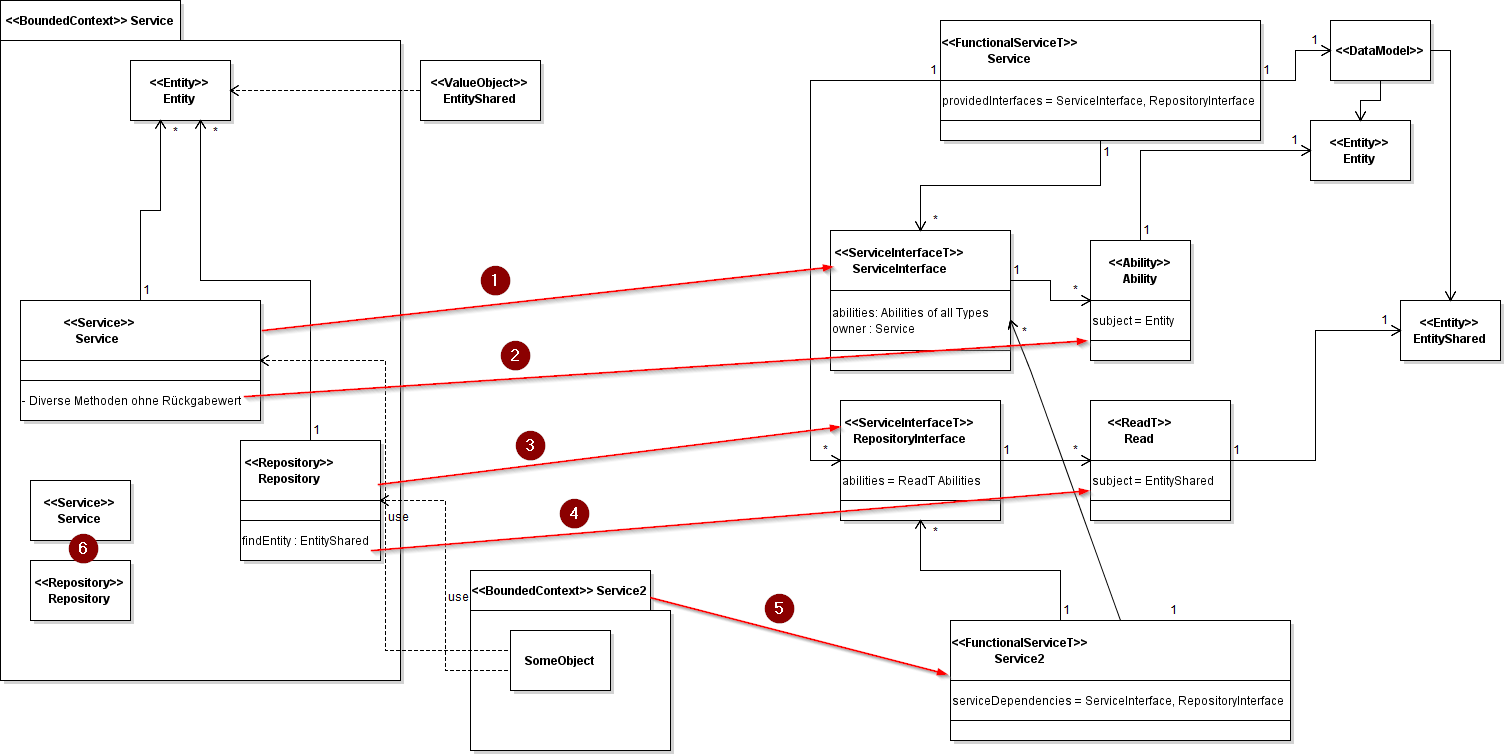
\includegraphics[width=\textwidth]{Bilder/servicesAndRepos.png}
\caption{Transformation von Repositories und Services}
\end{figure}
\section{Umgang mit Aggregaten}
Hier wird beschrieben wie mit Aggregaten umgegangen wird, also pack beshjjd
\begin{figure}
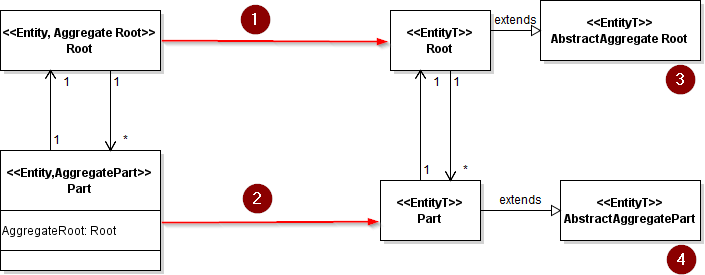
\includegraphics[width=\textwidth]{Bilder/aggregates_rules_explained.png}
\caption{Transformation von Aggregaten}
\end{figure}
\section{Tabellarischer Überblick über Regeln}
\begin{tabular}{*5l}    \toprule
\emph{name} & \emph{foo} &&&  \\\midrule
Models    & A  & B  & C  & D  \\ 
 Model $X$ & X1 & X2 & X3 & X4\\ 
 Model $Y$ & Y1 & Y2 & Y3 & Y4\\\bottomrule
 \hline
\end{tabular}

\section{Grafische Darstellung der Regeln}


- Packages werden nicht transformiert, da in AJIL kein entsprechendes Konzept existiert. Überlegung hier wäre ein Package ein DataModel, aber es können Beziehungen zwischen Elementen in verschiedenen Packages bestehen, nicht zwischen Elementen von DataModels.

\chapter{Implementierung des Konzepts}
\begin{figure}
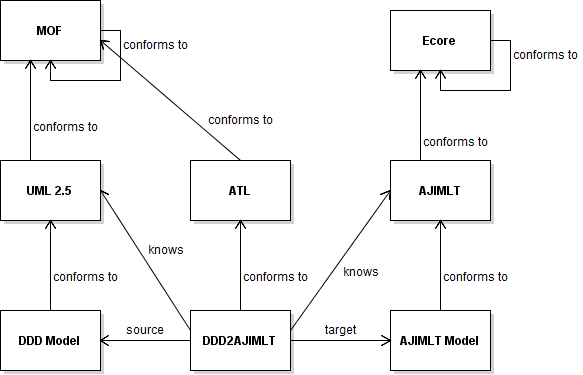
\includegraphics[width=\textwidth]{Bilder/transformationModelOverview.png}
\caption{Transformationsmodellübersicht}
\end{figure}
\section{Auswahl einer geeigneten Transformationstechnologie}
\subsection{Kriterien}
\subsection{Optionen}
\subsection{Entscheidung}
\section{Formulierte Regeln}
\section{Ausführung}
\section{Evaluation anhand eines Domänenmodells aus der Praxis}
\chapter{Abschluss}
\label{chap:zusammenfassung}
\section{Zusammenfassung}
\section{Fazit}
\section{Ausblick}
	

% Abkürzungsverzeichnis ins Inhaltsverzeichnis aufnehmen und mit Inhalt füllen
\cleardoublepage\phantomsection\addcontentsline{toc}{chapter}{Abkürzungsverzeichnis}
\chapter*{Abkürzungsverzeichnis}
	\begin{acronym}[NMWC] % längste Abkürzung steht in eckigen Klammern
    	\setlength{\itemsep}{-\parsep} % geringerer Zeilenabstand
    		\acro{ajil}[AjiL]{\textit{Ajil Modeling Language}}
		\acro{ddd}[DDD] {\textit{Domain-driven Design}}
		\acro{dsl}[DSL]{\textit{Domain Specific Language}}
		\acro{dsml}[DSML]{\textit{Domain Specific Modelling Language}}
		\acro{edm}[EDM]{\textit{Example-driven Modelling}}
		\acro{gpl}[GPL]{\textit{General Purpose Language}}
		\acro{idial}[IDiAL]{\textit{Institut für die Digitalisierung von Arbeits- und Lebenswelten}}
		\acro{mdsd}[MDSD]{\textit{Model Driven Software Development}}
		\acro{mof}[MOF]{\textit{Meta Object Facility}}
		\acro{msa}[MSA]{\textit{Microservice Architecture}}
		\acro{omg}[OMG]{\textit{Object Management group}}
		\acro{rest}[REST]{\textit{Representational State Transfer }}
		\acro{soa}[SOA]{\textit{Service Oriented Architecture}}
		\acro{sus}[SuS]{\textit{System Under Study}}
		\acro{uml}[UML] {\textit{Unified Modeling Language}}
\end{acronym}

\newpage{}

% Weitere Verzeichnisse ins Inhaltsverzeichnis aufnehmen
\cleardoublepage\phantomsection\addcontentsline{toc}{chapter}{Abbildungsverzeichnis}
\listoffigures

\newpage{}

\cleardoublepage\phantomsection\addcontentsline{toc}{chapter}{Tabellenverzeichnis}
\listoftables

\lstlistoflistings 
	
% Literaturverzeichnis setzen
\bibliographystyle{alphadin}
\bibliography{bib}
	
% Eidesstattliche Erklärung. ACHTUNG: Korrekten Text bitte unbedingt vorab mit Studienbüro klären!
\chapter*{Eidesstattliche Erklärung}
\thispagestyle{empty}
\textbf{ACHTUNG: Korrekten Text bitte unbedingt vorab mit Studienbüro klären!}\\
Hiermit versichere ich gemäß § 18 Abs. 5 der Bachelor-Prüfungsordnung des Studiengangs Informatik aus dem Jahr 2013, dass ich die  vorliegende Arbeit selbstständig angefertigt und mich keiner fremden Hilfe bedient, sowie keine anderen als die angegebenen Quellen und Hilfsmittel benutzt habe. Alle Stellen, die wörtlich oder sinngemäß veröffentlichten oder nicht veröffentlichten Schriften und anderen Quellen entnommen sind, habe ich als solche kenntlich gemacht. Diese Arbeit hat in gleicher oder ähnlicher Form noch keiner Prüfungsbehörde vorgelegen.

\vspace{1\baselineskip}%
Dortmund, \fhdopaperdate \hfill \fhdopaperauthor
\end{document}